\documentclass[12pt]{article} % Default font size is 12pt, it can be changed here
\usepackage[portuguese]{babel}
\usepackage[utf8]{inputenc}
\usepackage[T1]{fontenc}
\usepackage{color}
\usepackage{indentfirst}

\usepackage{geometry} % Required to change the page size to A4
\geometry{a4paper} % Set the page size to be A4 as opposed to the default US Letter

\usepackage{graphicx} % Required for including pictures

% (1) choose a font that is available as T1
% for example:
\usepackage{lmodern}

% (2) specify encoding
\usepackage[T1]{fontenc}

% (3) load symbol definitions
\usepackage{textcomp}
\usepackage{float} % Allows putting an [H] in \begin{figure} to specify the exact location of the figure
\usepackage{wrapfig} % Allows in-line images such as the example fish picture

\usepackage{listings} % Para codigo cenas
\usepackage{array}
\usepackage{url}
\linespread{1.2} % Line spacing

\graphicspath{{./Pictures/}} % Specifies the directory where pictures are stored
\usepackage{fancyhdr}
\pagestyle{fancy}

\begin{document}
\lhead{Sistemas Distribuídos}
\rhead{Projecto 1}
%--------------------------------------------------------------------------
%	TITLE PAGE
%-------------------------------------------------------------------------

\begin{titlepage}

\newcommand{\HRule}{\rule{\linewidth}{0.5mm}} % Defines a new command for the horizontal lines, change thickness here

\center % Center everything on the page

\textsc{\LARGE Universidade de Coimbra}\\[1.5cm] % Name of your university/college
\textsc{\Large Licenciatura Engenharia Informática\\2013-2014}\\[0.5cm] % Major heading such as course name

\HRule \\[0.4cm]
{\huge \bfseries Sistemas Distribuídos - Project 1}\\[0.4cm] % Title of your document
\HRule \\[1.5cm]

\begin{minipage}{0.8\textwidth}

\begin{flushleft} \large
\emph{Autores:}\\
Gustavo \textsc{Fresco} - Nº2006105289\\ % Your name
Bruno \textsc{Martins} - Nº2007183389
\end{flushleft}

\end{minipage}

\begin{minipage}{0.4\textwidth}
\begin{flushright} \large
\end{flushright}
\end{minipage}\\[4cm]

{\large \today}\\[3cm] % Date, change the \today to a set date if you want to be precise
\vfill % Fill the rest of the page with whitespace

\end{titlepage}

%--------------------------------------------------------------------------
%	TABLE OF CONTENTS
%--------------------------------------------------------------------------
\tableofcontents % Include a table of contents



\newpage % Begins the essay on a new page instead of on the same page as the table of contents 

%--------------------------------------------------------------------------
%	INTRODUCTION
%--------------------------------------------------------------------------

\section{Introdução} % Major section
\label{sec:intro}
O presente relatório destina-se a apresentar a descrição do projecto 1 da cadeira de Sistemas Distribuídos intitulada \emph{IdeaBroker – Idea Management and Trading}.\\

Ideias são um conceito poderoso. A maneira pela qual eles são organizados na Web não é a melhor, pois raramente é estruturado. Este projeto tem como objetivo organizar as idéias de uns contra os outros, com a capacidade de fornecer aos usuários uma visão geral sobre um tema específico, bem como uma indicação de quanto cada ideia vale a pena.\\

Ideias são submetidos pelos usuários, e outros usuários são capazes de concordar e discordar com essas ideias, submetendo os argumentos a favor e contra. Tais argumentos são, naturalmente, as ideias também. Dessa forma, ideias, pensamentos e opiniões são significativamente ligados uns aos outros (ao contrário dos botões atualmente típicos que fornecem nenhum raciocínio). - \textbf{Figura \ref{figure1}.}

\begin{figure}[!ht]
  	\centering
  	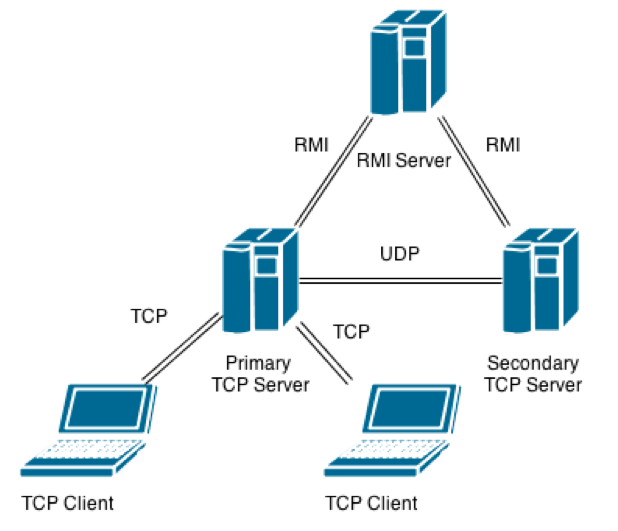
\includegraphics[scale=0.5]{figure1.png}
  	\caption{Visão Global da Arquitectura}
	%\vspace{2cm}
	\label{figure1}
\end{figure}


%--------------------------------------------------------------------------
%	INTERNAL ARCHITECTURE
%--------------------------------------------------------------------------
\section{Internal architecture}
\label{sub:internal}
O esquema abaixo apresentado procura descrever de forma simples a arquitetura desenvolvida:
\begin{figure}[!ht]
  	\centering
  	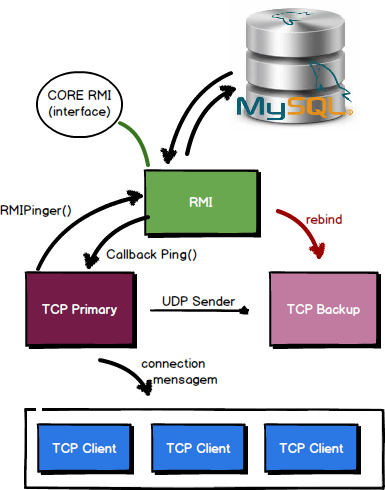
\includegraphics[scale=0.7]{sytem_arquitecture.png}
  	\caption{Arquitectura do Sistema}
	%\vspace{2cm}
	\label{figure2}
\end{figure}
%\newpage
%\vspace{0.5cm}

Esta aplicação encontra-se subdividida numa série de classes, cada uma responsável por integrar esta aplicação num todo coerente, onde se destacam:

\begin{description}
	\item[RMIServer:] \hfill \\
	Dentro da classe \textbf{RMIServer} encontram-se os métodos essenciais da aplicação: registo, login, createTopic, listAllTopics, listOwnIdeas, viewSharesFromIdea, etc. Dentro do RMIServer é executado o callback, que chama o método Ping() para verificação de ligação, caso o servidor a que este se encontra a fazer callback caia, o RMIServer irá então realizar \textbf{rebind()} para o servidor Backup. Relativamente as threads, o RMI tem a sua própria thread para executar. 
	\item[CoreRMI:] \hfill \\
	O CoreRMI é a nossa interface dos métodos existentes dentro da RMIServer.
	\item[TCPServer:] \hfill \\
	Existe duas threads dentro do TCPServer: uma a  pingar para o RMI e a outra a enviar pings através do UDP para o BackupServer.
	\item[BackupServer:] \hfill \\
	Dentro desta classe encontra-se o servidor secundário TCP, que se encontra à escuta, à espera que o servidor TCP Principal caía.
	\item[TCPClient:] \hfill \\
	Este cliente estabelece a ligação com o servidor através de Sockets TCP (recorrendo a streams de dados) promovendo não só a construção dos menus (menu de login, inicial, etc.) como também a arquitetura da aplicação melhorando, deste modo, a comunicabilidade com o servidor. É responsável por providenciar informação e dados através da criação de mensagens e pelo envio de imagens, como também requisita serviços à aplicação, como por exemplo listar ideias existentes, ou comprar shares.
\end{description}

Estes objetos são responsáveis por estabelecer grande parte da interoperabilidade desta aplicação embora sejam necessárias as restantes classes que suportam a estrutura por detrás deste sistema.\\ 




Relativamente ao armazenamento de dados na Base de Dados, foram criadas as tabelas:
\begin{description}
	\item[Person:] \hfill \\
	\textbf{id\_person, login, pass, email, money, online}\\
	A tabela \emph{Person} é a responsável por armazenar os dados dos users, assim como também a quantidade de dinheiro que possui (10000 por default) e tem um campo \underline{Online} que é um boolean que indica se este se encontra online ou não no sistema.
	
	\item[Ideias:] \hfill \\
	\textbf{id\_ideia, id\_person, description, attach}\\
	A tabela \textbf{Ideias} além de ter o seu próprio id, também guarda o id da pessoa responsável pela mesma. Tem também um campo com uma breve descrição e um campo attach que é um \textbf{BLOB}, no qual são guardados os ficheiros de anexo.
	\item[Shares:] \hfill \\
	\textbf{id\_person, id\_ideia, quantidade, price}\\
	A tabela \textbf{Shares} é a responsável pela ligação entre as shares das ideias e da respectiva pessoa que a detém. Tem um campo destinado à quantidade de shares e o seu preço.
	\item[Transactions:] \hfill \\
	\textbf{id\_transaction, id\_ideia, id\_person,	quantidade, transaction\_price, status}\\
	Na \textbf{Transactions} é registado as transações de ideias entre as diversas pessoas, bem como o preço a que esta foi transacionada e o seu status (se foi completado ou não).
	\item[Relation:] \hfill \\
	\textbf{id\_ideia1, id\_ideia2, value}\\
	A tabela \textbf{Relation} faz a gestão entre as relações entre diferentes ideias e o valor da sua relação (1 - Positiva, 0 - Neutra, -1 - Negativa)
	\item[Ideias\_Topic:] \hfill \\
	\textbf{id\_topic, id\_ideia}\\
	A tabela \textbf{Ideias\_Topic} é uma entidade fraca de ligação entre as tabelas \emph{ideas} e \emph{topic}
	\item[Topic:] \hfill \\
	\textbf{id\_topic, description}\\
	A tabela \textbf{Topic} armazena além do seu respectivo ID, uma breve descrição da mesma.
\end{description}


\begin{figure}[ht]
  	\centering
  	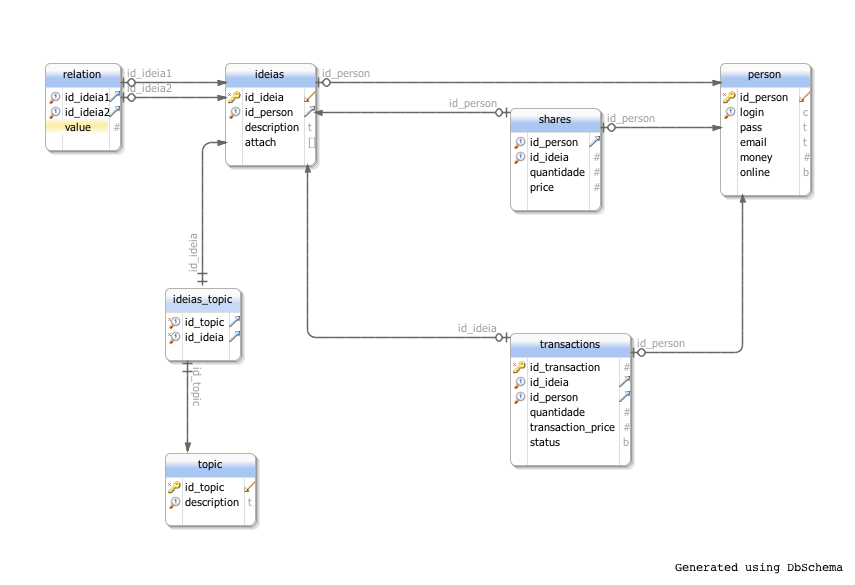
\includegraphics[scale=0.5]{ERdiagram.png}
  	\caption{Diagrama Entidade Relacionamento}
	%\vspace{2cm}
	\label{figure3}
\end{figure}

\-
\pagebreak


%--------------------------------------------------------------------------
%	DATA MODEL
%--------------------------------------------------------------------------
\section{Data model} % 
\label{sec:data}
O seguinte diagrama representa o nosso esquema de Data Model.

\begin{figure}[!ht]
  	\centering
  	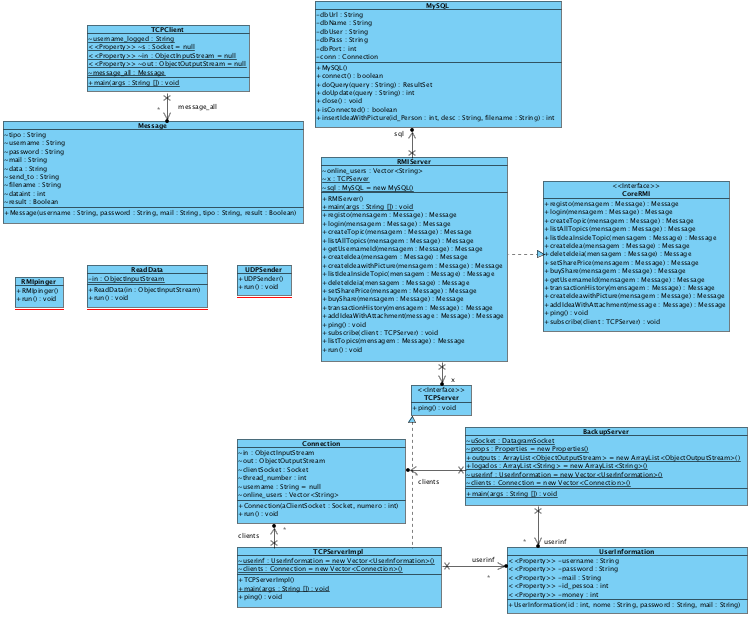
\includegraphics[scale=0.6]{ClassDiagram.png}
  	\caption{Data Diagram}
	%\vspace{2cm}
	\label{figure4}
\end{figure}

A comunicação entre client-server pressupõe uma eficiente troca de dados que podem ser ‘transmitidos’ diretamente através de Sockets (TCP). 
Estruturámos a informação de forma eficiente e intuitiva construindo diversas classes capazes de representar este modelo de dados. Devido a esta separação em objetos das mensagens a transmitir entre as entidades executantes, optámos por utilizar ObjectStreams (para Sockets TCP) salvaguardando toda essa informação em ficheiros de objetos garantindo, assim, a fiabilidade e integridade dos dados em trânsito (Message).





%--------------------------------------------------------------------------
%	Protocol Specification (TCP, UDP, RMI)
%--------------------------------------------------------------------------
\section{Protocol Specification (TCP, UDP, RMI)} % 
\label{sec:protocal_specs}

\subsection{TCP}
O servidor cria um ServerSocket, bloqueia no método accept e espera novos clientes. Quando um cliente se liga ao servidor, este estabelece um socket de comunicação com o mesmo e cria uma nova thread para “tratar” desse cliente. Desta forma, temos sempre o main bloqueado no listenSocket.accept à espera de novos clientes e preparado para criar uma thread por cliente (cada um tem a sua, Servidor Multithread).\\
Os métodos de que o servidor precisa para tratar dos pedidos de um cliente TCP estão criados no RMI Server. Quando termina de efectuar a acção requisitada pelo cliente, ela envia o resultado para o mesmo através de DataStream S.


\subsection{UDP}
A conexão UDP é estabelecida no início do funcionamento da aplicação de modo a assegurar o permanente controlo do estado de cada das entidades que supervisionam a gestão deste serviço. A diferença básica entre o UDP e o TCP é o fato de que o TCP ser um protocolo orientado à conexão e, portanto, inclui vários mecanismos para iniciar, manter e encerrar a comunicação, negociar tamanhos de pacotes, detectar e corrigir erros, evitar congestionamento do fluxo e permitir a retransmissão de pacotes corrompidos, independente da qualidade do meio físicos. No UDP não existem verificações, nem confirmações. 
É portanto uma escolha adequada para fluxos de dados em tempo real, especialmente aqueles que admitem perda ou corrompimento de parte de seu conteúdo.


\subsection{RMI}
O Java RMI(Remote Method Invocation) usa uma metodologia diferente da do TCP. Ao contrário deste não é estabelecido directamente um canal de comunicação como no TCP em que o servidor está a escuta num determinado porto e para cada cliente cria um socket.
Especificamente, neste projecto o RMI é o nosso main-server, sendo este responsável pelos métodos existentes em toda a sua envolvente.



%--------------------------------------------------------------------------
%	Architecture of File Transmission
%--------------------------------------------------------------------------
\section{Architecture of File Transmission}
\label{sec:archi}
O envio de ficheiros no nosso sistema foi feito recorrendo ao \emph{blob} na base de dados MySql. A base de dados, na tabela \emph{Ideias} tem um campo \emph{attach}, no qual está sendo armazenado os ficheiros pretendidos pelo utilizador. O utilizador ao introduzir uma ideia, é-lhe perguntado se este pretende associar um ficheiro a esta e de seguida coloca o path do ficheiro. Para fazer download de um attachment, o utilizador escolha mediante a apresentação da listagem de \emph{ideias}, aquele que pretende guardar. Este será guardado na raiz da aplicação de onde o programa se encontra a ser executado.


%--------------------------------------------------------------------------
%	Exception Handling
%--------------------------------------------------------------------------
\section{Exception Handling}
\label{sec:except}

No que toca a tratamentos de excepção, foi assegurado que um Cliente reconecta ao mesmo servidor em caso de falha temporária do TCPServer (através de um tempo de espera), sendo a falha transitória e transparente para o usuário final.
Através do uso de base de dados, o TCPClient não perde a ideia que está sendo escrita.
O TCPServer reconecta em caso de perda de conectividade com o RMIServer e 
a falha transitória da RMIServer é transparente para o usuário final.
Também houve o cuidado da verificação e foi assegurado que não existem ideias duplicadas, mesmo em cenários de entrega.

\subsection{A nível de Base de Dados}
O tratamento de erros do nosso MySQL é baseado em condições, que por sua vez, são nomeadas e preparadas para serem executadas mediante ao atendimento de tais condições. 
Além de tratarmos a violação de chaves primárias, foi tido em conta que os ids não assumam valores nulos (NULL), assim como houve um cuidado para que estes fossem auto-incrementáveis. Ao definir corretamente todas as relações e entidades fracas, foi possível haver um relacionamento directo entre entidades de diferentes campos (nomeadamente \emph{id\_person} na tabela \emph{person} com o \emph{id\_person} da tabela \emph{ideias}). Foi dado \textbf{cascade} em operações de \emph{update} e \emph{delete}, para que as ligações entre tabelas não fosse quebrada. Assim conseguimos garantir que ao apagar um \emph{ideia}, a tabela de relação com uma share é também destruída. 


\subsection{TCP}
De modo a tornar esta aplicação ao mesmo tempo transparente a erros e eficiente no seu tratamento procurámos controlar as exceções provenientes dos mecanismos de conexão (Sockets, RMI registry, etc.). Estes problemas advêm de falhas de ligação entre o servidor e o cliente, de uma ruptura do socket TCP, etc.
Implementámos diversas rotinas para gerir estas exceções (try/catch (IO Exception, Remote Exception)) em ambas as ‘extremidades’ da aplicação. As threads responsáveis por estas funções (ConnectBackupServer, UDP) permitem não só isolar o tratamento destas situações, podendo o cliente continuar a usar a aplicação (com algumas restrições), como também restabelecer as ligações entre as entidades executantes ou, em caso de insucesso, ativar um backup. 
Quando o servidor deixa de funcionar correctamente, vai ser detectada uma falha. O cliente irá então tentar voltar a conectar-se, sendo a função udpsender() a responsável pelas tentativas.
Na tentativa do Cliente se conectar ao Servidor, este efetua uma espera de um intervalos de 3 segundos entre cada tentativa de conexão. Entretanto, caso o cliente tente realizar algum pedido, a thread destinada à escrita de teclado fica bloqueada até este realizar re-connect.

\subsection{RMI}
No RMI foram dados os mesmos tratamentos de exceção utilizados no TCP.


\pagebreak

%--------------------------------------------------------------------------
%	FailOver
%--------------------------------------------------------------------------
\section{FailOver}
\label{sec:failover}
O fail-over pressupõe a existência de dois servidores (primary e backup -> tipo 1 e 2 respetivamente) que comunicam entre si através de um canal UDP. Só assim é possível controlar o estado (ativo/inativo) de cada uma das entidades e efetuar a troca em caso de necessidade. Para tal, operámos um mecanismo de ping (3s) iniciado pelo servidor secundário que providencia informação essencial na gestão de erros. 
Implementámos uma thread com uma duração de 5 segundos que corresponde ao tempo máximo de delay aceite pela aplicação. Se durante esse período a ‘entidade gestora’ em utilização não comunicar, os clientes serão redirecionados para o servidor secundário que assumirá o papel de principal.

\begin{figure}[!ht]
	\centering
		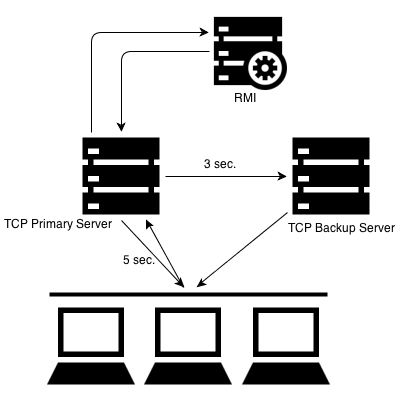
\includegraphics[scale=0.6]{failover.png}
	\caption{Esquema de FailOver}
	\label{fig:Pictures_failover}
\end{figure}

\pagebreak
%--------------------------------------------------------------------------
%	Strict Order Implementation
%--------------------------------------------------------------------------
\section{Strict Order Implementation}
\label{sec:strict}
Para implementar o nosso projecto, começamos por criar as respectivas ligações e a criação dos clientes. Inicialmente criamos somente o TCP Server, no qual colocamos todas as operações necessárias e mais tarde passamos estas mesmas para o servidor RMI. Foi também criado uma interface \emph{CORERmi}, na qual temos a declaração das funções necessárias ao longo da aplicação.
Relativamente ao armazenamento de dados, optamos numa primeira instância por recorrer a ficheiros (tipo vector), mas logo percebemos que para existir uma maior segurança e fiabilidade de armazenamento de dados a melhor operação era recorrer a uma base de dados, nomeadamente o \emph{MySQL}. Relativamente à base de dados, foi feito uma análise cuidada das tabelas, campos e ligações a usar de acordo com as nossas necessidades.

Por fim, foi criado o servidor backup e a sua respectiva ligação UDP. Somente no fim da implementação dos mecanismos de \textbf{FailOver} e dos mecanismos de \textbf{tratamento de excepções}, é que nos concentramos na parte dos objectos / requisitos funcionais.


\pagebreak
%--------------------------------------------------------------------------
%	Description of tests (Table with Pass/Fail)
%--------------------------------------------------------------------------
\section{Description of tests (Table with Pass/Fail)} % (fold)
\label{sec:Tests}
Foram feitos diversos testes nas diversas funcionalidades da aplicação, de modo a assegurar a robustez da aplicação garantindo, assim, um sistema seguro e eficiente, procurámos testá-lo minuciosamente.

%%%%%%%%%%%%%%%%%%%%%%%%%%%%%%%%%%%%%%%%%%%%%%%%---------------REGISTER
\subsection{Teste de Registo}
\begin{table}[ht!]
	\begin{tabular}{|c|p{4cm}|p{4cm}|p{3cm}|p{1cm}|}
		\hline
		\multicolumn{5}{|l|}{\textbf{Test Name}: Registar}\\
		\hline
		\multicolumn{5}{|l|}{\textbf{Description}: Registo do cliente na BD da aplicação}\\
		\hline
		\multicolumn{5}{|p{14,5cm}|}{\textbf{Prerequisites}: O cliente tem de entrar na aplicação e escolhe a opção REGISTAR}\\
		\hline
		\multicolumn{5}{|l|}{\textbf{Setup}: O cliente cria uma nova conta}\\
		\hline
		\textbf{Step} & \textbf{Operator Action} & \textbf{Expected Results} & \textbf{Observed Results} & \textbf{Pass / Fail}\\
		\hline
		1 & Escolhe a opção Registar & Sistema abre os campos de registo & São os esperados & PASS\\
		\hline
		2 & Inserir username, password e email & Sistema aceita dados e guarda na BD ou rejeita caso o username escolhido já esteja a ser utilizado & São os esperados & PASS\\
		\hline
	\end{tabular}
\end{table}
\pagebreak


%%%%%%%%%%%%%%%%%%%%%%%%%%%%%%%%%%%%%%%%%%%%%%%%---------------LOGIN
\subsection{Teste de Login}
\begin{table}[ht!]
	\begin{tabular}{|c|p{4cm}|p{4cm}|p{3cm}|p{1cm}|}
		\hline
		\multicolumn{5}{|l|}{\textbf{Test Name}: Login}\\
		\hline
		\multicolumn{5}{|l|}{\textbf{Description}: Identificação do cliente}\\
		\hline
		\multicolumn{5}{|p{14,5cm}|}{\textbf{Prerequisites}: Cliente tem de ter uma conta criada na aplicação}\\
		\hline
		\multicolumn{5}{|l|}{\textbf{Setup}: O cliente insere a sua pass e username para usar a sua conta}\\
		\hline
		\textbf{Step} & \textbf{Operator Action} & \textbf{Expected Results} & \textbf{Observed Results} & \textbf{Pass / Fail}\\
		\hline
		1 & Inserir username, password & Sistema aceita dados se essa conta existir & São os esperados & PASS\\
		\hline
	\end{tabular}
\end{table}
\pagebreak

%%%%%%%%%%%%%%%%%%%%%%%%%%%%%%%%%%%%%%%%%%%%%%%%---------------IDEIA
\subsection{Teste de Submissão de Ideia}
\begin{table}[ht!]
	\begin{tabular}{|c|p{4cm}|p{4cm}|p{3cm}|p{1cm}|}
		\hline
		\multicolumn{5}{|l|}{\textbf{Test Name}: Teste de Submissão de Ideia}\\
		\hline
		\multicolumn{5}{|p{14,5cm}|}{\textbf{Description}: É testada a funcionalidade de introduzir ideia}\\
		\hline
		\multicolumn{5}{|p{14,5cm}|}{\textbf{Prerequisites}: O utilizador tem que já estar registado e já devem existir ideias}\\
		\hline
		\multicolumn{5}{|p{14,5cm}|}{\textbf{Setup}: O servidor irá fazer handle das ideias}\\
		\hline
		\textbf{Step} & \textbf{Operator Action} & \textbf{Expected Results} & \textbf{Observed Results} & \textbf{P / F}\\
		\hline
		1 & logar User & Login efectuado com sucesso! & Nada apontar & PASS\\
		\hline
		2 & User acede ao menu e escolhe a opção 3 & aparece o passo seguinte & antes de escolher a opção, aparece uma listagem de opções & PASS\\
		\hline
		3 & Introduz a conteúdo da ideia & Pergunta se deseja introduzir anexo & nada apontar & PASS\\
		\hline
		4 & Escolhe a opção de sim relativamente ao anexo & Passa ao passo seguinte & é introduzido a path do anexo & PASS\\
		\hline
		5 & --- & Passa À seguinte pergunta relativamente a adicionar a ideia a um tópico & pergunta se deseja introduzir um novo tópico ou usar os existentes & PASS\\
		\hline
		6 & Escolhe a opção de usar tópicos existentes & Lista todos os tópicos existentes & nada apontar & PASS\\
		\hline
		7 & Vai introduzir os tópicos 1 e 2 e por fim clica em 0 para finalizar & Ir pedindo mais tópicos enquanto não se clica na tecla 0 & É introduzida a associação da ideia com o tópico, com sucesso & PASS\\
		\hline
	\end{tabular}
\end{table}
\pagebreak



%%%%%%%%%%%%%%%%%%%%%%%%%%%%%%%%%%%%%%%%%%%%%%%%---------------CONECTAR A BACKUP
\subsection{Teste de Ligação ao Servidor Backup}
\begin{table}[ht!]
	\begin{tabular}{|c|p{4cm}|p{4cm}|p{3cm}|p{1cm}|}
		\hline
		\multicolumn{5}{|l|}{\textbf{Test Name}: Ligação ao Servidor Backup}\\
		\hline
		\multicolumn{5}{|l|}{\textbf{Description}: Teste de Ligação ao Backup}\\
		\hline
		\multicolumn{5}{|p{14,5cm}|}{\textbf{Prerequisites}: Cliente tem de ter uma conta criada na aplicação e devem estar os dois servidores a correr (Principal e Backup). Será feita uma ligação normal entre cliente TCP e Servidor TCP. De seguida será quebrada a ligação do servidor principal TCP, esperando assim que o cliente se reconecte ao servidor backup}\\
		\hline
		\multicolumn{5}{|l|}{\textbf{Setup}: Acesso normal À sua conta}\\
		\hline
		\textbf{Step} & \textbf{Operator Action} & \textbf{Expected Results} & \textbf{Observed Results} & \textbf{Pass / Fail}\\
		\hline
		1 & Inserir username, password & Sistema aceita dados se a conta existir & São os esperados & PASS\\
		\hline
		2 & O servidor principal é desligado & Existe um período de espera da parte do cliente até este se ligar ao servidor backup, podendo ter existido uma pequena baixa da parte do principal & O servidor principal não vem à vida dentro o tempo de espera & PASS\\
		\hline
		3 & ---- & Ligação feita ao servidor backup & São os esperados & PASS\\
		\hline
	\end{tabular}
\end{table}




\newpage
%--------------------------------------------------------------------------
%	Manual de Instalação
%--------------------------------------------------------------------------
\section{Manual de Instalação}
\label{sec:install}
Para correr a aplicação irá necessitar dos seguintes requisitos:
\begin{itemize}
	\item Java 5 ou Superior
	\item Servidor com MySQL com a respectiva base de dados (o script de criação da base de dados encontra-se na raiz deste projecto dentro do ficheiro \emph{sd1\_2013.sql})
\end{itemize}

Após reunidos todos requisitos necessários, é necessário que o MySQL esteja a correr dentro da própria (localhost), ou no caso que esteja se encontre noutra máquina, que seja definido o respectivo IP e porta.
Como foi mencionado anteriormente, deve-se correr o script \emph{sd1\_2013.sql} que contem todas as tabelas criadas bem como alguns dados.
Por fim, deve-se executar-se por esta ordem a execução de Servidores da máquina:

\begin{itemize}
	\item 1 - RMIServer.java
 	\item 2 - TCPServer.java
	\item 3 - BackupServer.java
	\item 4 - TCPClient.java
\end{itemize}
Relativamente ao IP de máquina onde os servidores e o cliente estão a correr, existe um ficheiro intitulado \textbf{Property} onde se pode alterar os endereços e as portas onde estes vão estar a correr.

\begin{verbatim}
tcpip1=127.0.0.1
tcpip2=127.0.0.1
tcpserverPort=7000
tcpserverPortAux=7002
tcpbserverPort=7001
udpPort=5000
rmiServerip=127.0.0.1
rmiServerPort1=1099
rmiServerPort2=6001
\end{verbatim}


E... pronto! É só escolher as operações pretendidas!



\end{document}